\documentclass[1p]{elsarticle_modified}
%\bibliographystyle{elsarticle-num}

%\usepackage[colorlinks]{hyperref}
%\usepackage{abbrmath_seonhwa} %\Abb, \Ascr, \Acal ,\Abf, \Afrak
\usepackage{amsfonts}
\usepackage{amssymb}
\usepackage{amsmath}
\usepackage{amsthm}
\usepackage{scalefnt}
\usepackage{amsbsy}
\usepackage{kotex}
\usepackage{caption}
\usepackage{subfig}
\usepackage{color}
\usepackage{graphicx}
\usepackage{xcolor} %% white, black, red, green, blue, cyan, magenta, yellow
\usepackage{float}
\usepackage{setspace}
\usepackage{hyperref}

\usepackage{tikz}
\usetikzlibrary{arrows}

\usepackage{multirow}
\usepackage{array} % fixed length table
\usepackage{hhline}

%%%%%%%%%%%%%%%%%%%%%
\makeatletter
\renewcommand*\env@matrix[1][\arraystretch]{%
	\edef\arraystretch{#1}%
	\hskip -\arraycolsep
	\let\@ifnextchar\new@ifnextchar
	\array{*\c@MaxMatrixCols c}}
\makeatother %https://tex.stackexchange.com/questions/14071/how-can-i-increase-the-line-spacing-in-a-matrix
%%%%%%%%%%%%%%%

\usepackage[normalem]{ulem}

\newcommand{\msout}[1]{\ifmmode\text{\sout{\ensuremath{#1}}}\else\sout{#1}\fi}
%SOURCE: \msout is \stkout macro in https://tex.stackexchange.com/questions/20609/strikeout-in-math-mode

\newcommand{\cancel}[1]{
	\ifmmode
	{\color{red}\msout{#1}}
	\else
	{\color{red}\sout{#1}}
	\fi
}

\newcommand{\add}[1]{
	{\color{blue}\uwave{#1}}
}

\newcommand{\replace}[2]{
	\ifmmode
	{\color{red}\msout{#1}}{\color{blue}\uwave{#2}}
	\else
	{\color{red}\sout{#1}}{\color{blue}\uwave{#2}}
	\fi
}

\newcommand{\Sol}{\mathcal{S}} %segment
\newcommand{\D}{D} %diagram
\newcommand{\A}{\mathcal{A}} %arc


%%%%%%%%%%%%%%%%%%%%%%%%%%%%%5 test

\def\sl{\operatorname{\textup{SL}}(2,\Cbb)}
\def\psl{\operatorname{\textup{PSL}}(2,\Cbb)}
\def\quan{\mkern 1mu \triangleright \mkern 1mu}

\theoremstyle{definition}
\newtheorem{thm}{Theorem}[section]
\newtheorem{prop}[thm]{Proposition}
\newtheorem{lem}[thm]{Lemma}
\newtheorem{ques}[thm]{Question}
\newtheorem{cor}[thm]{Corollary}
\newtheorem{defn}[thm]{Definition}
\newtheorem{exam}[thm]{Example}
\newtheorem{rmk}[thm]{Remark}
\newtheorem{alg}[thm]{Algorithm}

\newcommand{\I}{\sqrt{-1}}
\begin{document}

%\begin{frontmatter}
%
%\title{Boundary parabolic representations of knots up to 8 crossings}
%
%%% Group authors per affiliation:
%\author{Yunhi Cho} 
%\address{Department of Mathematics, University of Seoul, Seoul, Korea}
%\ead{yhcho@uos.ac.kr}
%
%
%\author{Seonhwa Kim} %\fnref{s_kim}}
%\address{Center for Geometry and Physics, Institute for Basic Science, Pohang, 37673, Korea}
%\ead{ryeona17@ibs.re.kr}
%
%\author{Hyuk Kim}
%\address{Department of Mathematical Sciences, Seoul National University, Seoul 08826, Korea}
%\ead{hyukkim@snu.ac.kr}
%
%\author{Seokbeom Yoon}
%\address{Department of Mathematical Sciences, Seoul National University, Seoul, 08826,  Korea}
%\ead{sbyoon15@snu.ac.kr}
%
%\begin{abstract}
%We find all boundary parabolic representation of knots up to 8 crossings.
%
%\end{abstract}
%\begin{keyword}
%    \MSC[2010] 57M25 
%\end{keyword}
%
%\end{frontmatter}

%\linenumbers
%\tableofcontents
%
\newcommand\colored[1]{\textcolor{white}{\rule[-0.35ex]{0.8em}{1.4ex}}\kern-0.8em\color{red} #1}%
%\newcommand\colored[1]{\textcolor{white}{ #1}\kern-2.17ex	\textcolor{white}{ #1}\kern-1.81ex	\textcolor{white}{ #1}\kern-2.15ex\color{red}#1	}

{\Large $\underline{12n_{0763}~(K12n_{0763})}$}

\setlength{\tabcolsep}{10pt}
\renewcommand{\arraystretch}{1.6}
\vspace{1cm}\begin{tabular}{m{100pt}>{\centering\arraybackslash}m{274pt}}
\multirow{5}{120pt}{
	\centering
	\includegraphics[width=112pt]{../../../GIT/diagram.site/Diagrams/png/2852_12n_0763.png}\\
\ \ \ A knot diagram\footnotemark}&
\allowdisplaybreaks
\textbf{Linearized knot diagam} \\
\cline{2-2}
 &
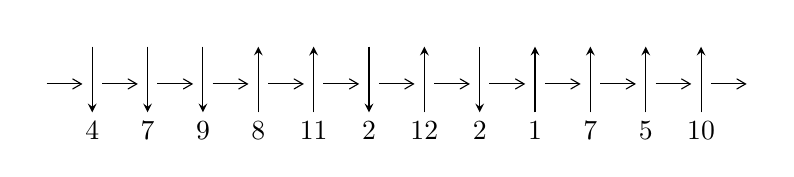
\begin{tikzpicture}[x=20pt, y=17pt]
	% nodes
	\node (C0) at (0, 0) {};
	\node (C1) at (1, 0) {};
	\node (C1U) at (1, +1) {};
	\node (C1D) at (1, -1) {4};

	\node (C2) at (2, 0) {};
	\node (C2U) at (2, +1) {};
	\node (C2D) at (2, -1) {7};

	\node (C3) at (3, 0) {};
	\node (C3U) at (3, +1) {};
	\node (C3D) at (3, -1) {9};

	\node (C4) at (4, 0) {};
	\node (C4U) at (4, +1) {};
	\node (C4D) at (4, -1) {8};

	\node (C5) at (5, 0) {};
	\node (C5U) at (5, +1) {};
	\node (C5D) at (5, -1) {11};

	\node (C6) at (6, 0) {};
	\node (C6U) at (6, +1) {};
	\node (C6D) at (6, -1) {2};

	\node (C7) at (7, 0) {};
	\node (C7U) at (7, +1) {};
	\node (C7D) at (7, -1) {12};

	\node (C8) at (8, 0) {};
	\node (C8U) at (8, +1) {};
	\node (C8D) at (8, -1) {2};

	\node (C9) at (9, 0) {};
	\node (C9U) at (9, +1) {};
	\node (C9D) at (9, -1) {1};

	\node (C10) at (10, 0) {};
	\node (C10U) at (10, +1) {};
	\node (C10D) at (10, -1) {7};

	\node (C11) at (11, 0) {};
	\node (C11U) at (11, +1) {};
	\node (C11D) at (11, -1) {5};

	\node (C12) at (12, 0) {};
	\node (C12U) at (12, +1) {};
	\node (C12D) at (12, -1) {10};
	\node (C13) at (13, 0) {};

	% arrows
	\draw[->,>={angle 60}]
	(C0) edge (C1) (C1) edge (C2) (C2) edge (C3) (C3) edge (C4) (C4) edge (C5) (C5) edge (C6) (C6) edge (C7) (C7) edge (C8) (C8) edge (C9) (C9) edge (C10) (C10) edge (C11) (C11) edge (C12) (C12) edge (C13) ;	\draw[->,>=stealth]
	(C1U) edge (C1D) (C2U) edge (C2D) (C3U) edge (C3D) (C4D) edge (C4U) (C5D) edge (C5U) (C6U) edge (C6D) (C7D) edge (C7U) (C8U) edge (C8D) (C9D) edge (C9U) (C10D) edge (C10U) (C11D) edge (C11U) (C12D) edge (C12U) ;
	\end{tikzpicture} \\
\hhline{~~} \\& 
\textbf{Solving Sequence} \\ \cline{2-2} 
 &
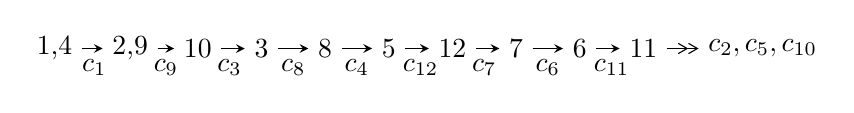
\begin{tikzpicture}[x=23pt, y=7pt]
	% node
	\node (A0) at (-1/8, 0) {1,4};
	\node (A1) at (17/16, 0) {2,9};
	\node (A2) at (17/8, 0) {10};
	\node (A3) at (25/8, 0) {3};
	\node (A4) at (33/8, 0) {8};
	\node (A5) at (41/8, 0) {5};
	\node (A6) at (49/8, 0) {12};
	\node (A7) at (57/8, 0) {7};
	\node (A8) at (65/8, 0) {6};
	\node (A9) at (73/8, 0) {11};
	\node (C1) at (1/2, -1) {$c_{1}$};
	\node (C2) at (13/8, -1) {$c_{9}$};
	\node (C3) at (21/8, -1) {$c_{3}$};
	\node (C4) at (29/8, -1) {$c_{8}$};
	\node (C5) at (37/8, -1) {$c_{4}$};
	\node (C6) at (45/8, -1) {$c_{12}$};
	\node (C7) at (53/8, -1) {$c_{7}$};
	\node (C8) at (61/8, -1) {$c_{6}$};
	\node (C9) at (69/8, -1) {$c_{11}$};
	\node (A10) at (11, 0) {$c_{2},c_{5},c_{10}$};

	% edge
	\draw[->,>=stealth]	
	(A0) edge (A1) (A1) edge (A2) (A2) edge (A3) (A3) edge (A4) (A4) edge (A5) (A5) edge (A6) (A6) edge (A7) (A7) edge (A8) (A8) edge (A9) ;
	\draw[->>,>={angle 60}]	
	(A9) edge (A10);
\end{tikzpicture} \\ 

\end{tabular} \\

\footnotetext{
The image of knot diagram is generated by the software ``\textbf{Draw programme}" developed by Andrew Bartholomew(\url{http://www.layer8.co.uk/maths/draw/index.htm\#Running-draw}), where we modified some parts for our purpose(\url{https://github.com/CATsTAILs/LinksPainter}).
}\phantom \\ \newline 
\centering \textbf{Ideals for irreducible components\footnotemark of $X_{\text{par}}$} 
 
\begin{align*}
I^u_{1}&=\langle 
-3.59010\times10^{543} u^{113}-8.27251\times10^{543} u^{112}+\cdots+3.57252\times10^{542} b-1.07356\times10^{547},\\
\phantom{I^u_{1}}&\phantom{= \langle  }-8.06333\times10^{546} u^{113}-1.86629\times10^{547} u^{112}+\cdots+7.43442\times10^{545} a-2.44436\times10^{550},\\
\phantom{I^u_{1}}&\phantom{= \langle  }u^{114}+3 u^{113}+\cdots+2274 u+2081\rangle \\
I^u_{2}&=\langle 
-4.10551\times10^{56} u^{39}+4.77048\times10^{57} u^{38}+\cdots+1.95140\times10^{54} b+9.86101\times10^{56},\\
\phantom{I^u_{2}}&\phantom{= \langle  }1.94943\times10^{56} u^{39}-2.22118\times10^{57} u^{38}+\cdots+1.95140\times10^{54} a-2.61580\times10^{56},\;u^{40}-12 u^{39}+\cdots-13 u+1\rangle \\
\\
\end{align*}
\raggedright * 2 irreducible components of $\dim_{\mathbb{C}}=0$, with total 154 representations.\\
\footnotetext{All coefficients of polynomials are rational numbers. But the coefficients are sometimes approximated in decimal forms when there is not enough margin.}
\newpage
\renewcommand{\arraystretch}{1}
\centering \section*{I. $I^u_{1}= \langle -3.59\times10^{543} u^{113}-8.27\times10^{543} u^{112}+\cdots+3.57\times10^{542} b-1.07\times10^{547},\;-8.06\times10^{546} u^{113}-1.87\times10^{547} u^{112}+\cdots+7.43\times10^{545} a-2.44\times10^{550},\;u^{114}+3 u^{113}+\cdots+2274 u+2081 \rangle$}
\flushleft \textbf{(i) Arc colorings}\\
\begin{tabular}{m{7pt} m{180pt} m{7pt} m{180pt} }
\flushright $a_{1}=$&$\begin{pmatrix}1\\0\end{pmatrix}$ \\
\flushright $a_{4}=$&$\begin{pmatrix}0\\u\end{pmatrix}$ \\
\flushright $a_{2}=$&$\begin{pmatrix}1\\u^2\end{pmatrix}$ \\
\flushright $a_{9}=$&$\begin{pmatrix}10.8459 u^{113}+25.1033 u^{112}+\cdots-11515.0 u+32879.0\\10.0492 u^{113}+23.1559 u^{112}+\cdots-10227.3 u+30050.4\end{pmatrix}$ \\
\flushright $a_{10}=$&$\begin{pmatrix}20.8951 u^{113}+48.2593 u^{112}+\cdots-21742.3 u+62929.3\\10.0492 u^{113}+23.1559 u^{112}+\cdots-10227.3 u+30050.4\end{pmatrix}$ \\
\flushright $a_{3}=$&$\begin{pmatrix}8.27906 u^{113}+18.6578 u^{112}+\cdots-5511.22 u+22301.8\\1.74357 u^{113}+3.90062 u^{112}+\cdots-1096.27 u+4622.46\end{pmatrix}$ \\
\flushright $a_{8}=$&$\begin{pmatrix}15.8478 u^{113}+36.5289 u^{112}+\cdots-16078.0 u+47458.1\\12.6154 u^{113}+29.0145 u^{112}+\cdots-12495.6 u+37500.0\end{pmatrix}$ \\
\flushright $a_{5}=$&$\begin{pmatrix}1.97516 u^{113}+4.35136 u^{112}+\cdots-598.296 u+4503.78\\-2.04245 u^{113}-4.70649 u^{112}+\cdots+2303.73 u-6285.34\end{pmatrix}$ \\
\flushright $a_{12}=$&$\begin{pmatrix}-0.754139 u^{113}-1.46500 u^{112}+\cdots-1218.31 u-1437.16\\1.46713 u^{113}+3.45524 u^{112}+\cdots-2212.82 u+4710.28\end{pmatrix}$ \\
\flushright $a_{7}=$&$\begin{pmatrix}-2.40049 u^{113}-5.98805 u^{112}+\cdots+5272.15 u-8510.38\\1.09194 u^{113}+2.32750 u^{112}+\cdots+159.454 u+2526.66\end{pmatrix}$ \\
\flushright $a_{6}=$&$\begin{pmatrix}-0.774473 u^{113}-2.15650 u^{112}+\cdots+3195.50 u-3458.59\\1.76349 u^{113}+3.93022 u^{112}+\cdots-844.537 u+4704.44\end{pmatrix}$ \\
\flushright $a_{11}=$&$\begin{pmatrix}13.2757 u^{113}+30.6061 u^{112}+\cdots-13426.7 u+39886.1\\7.22451 u^{113}+16.5415 u^{112}+\cdots-6672.28 u+21112.1\end{pmatrix}$\\&\end{tabular}
\flushleft \textbf{(ii) Obstruction class $= -1$}\\~\\
\flushleft \textbf{(iii) Cusp Shapes $= -27.2813 u^{113}-61.6278 u^{112}+\cdots+18528.3 u-75934.0$}\\~\\
\newpage\renewcommand{\arraystretch}{1}
\flushleft \textbf{(iv) u-Polynomials at the component}\newline \\
\begin{tabular}{m{50pt}|m{274pt}}
Crossings & \hspace{64pt}u-Polynomials at each crossing \\
\hline $$\begin{aligned}c_{1}\end{aligned}$$&$\begin{aligned}
&u^{114}-3 u^{113}+\cdots-2274 u+2081
\end{aligned}$\\
\hline $$\begin{aligned}c_{2},c_{6}\end{aligned}$$&$\begin{aligned}
&u^{114}+31 u^{112}+\cdots-8992 u+727
\end{aligned}$\\
\hline $$\begin{aligned}c_{3}\end{aligned}$$&$\begin{aligned}
&u^{114}- u^{113}+\cdots+7575 u+971
\end{aligned}$\\
\hline $$\begin{aligned}c_{4}\end{aligned}$$&$\begin{aligned}
&u^{114}-3 u^{113}+\cdots+677580 u+100759
\end{aligned}$\\
\hline $$\begin{aligned}c_{5},c_{11}\end{aligned}$$&$\begin{aligned}
&u^{114}+u^{113}+\cdots-32148 u+2295
\end{aligned}$\\
\hline $$\begin{aligned}c_{7}\end{aligned}$$&$\begin{aligned}
&u^{114}+2 u^{113}+\cdots+32727 u+2699
\end{aligned}$\\
\hline $$\begin{aligned}c_{8}\end{aligned}$$&$\begin{aligned}
&u^{114}+u^{113}+\cdots-789311 u+110833
\end{aligned}$\\
\hline $$\begin{aligned}c_{9},c_{12}\end{aligned}$$&$\begin{aligned}
&u^{114}+5 u^{113}+\cdots+925855 u+133141
\end{aligned}$\\
\hline $$\begin{aligned}c_{10}\end{aligned}$$&$\begin{aligned}
&u^{114}+2 u^{113}+\cdots-346643 u+24343
\end{aligned}$\\
\hline
\end{tabular}\\~\\
\newpage\renewcommand{\arraystretch}{1}
\flushleft \textbf{(v) Riley Polynomials at the component}\newline \\
\begin{tabular}{m{50pt}|m{274pt}}
Crossings & \hspace{64pt}Riley Polynomials at each crossing \\
\hline $$\begin{aligned}c_{1}\end{aligned}$$&$\begin{aligned}
&y^{114}-45 y^{113}+\cdots-156805222 y+4330561
\end{aligned}$\\
\hline $$\begin{aligned}c_{2},c_{6}\end{aligned}$$&$\begin{aligned}
&y^{114}+62 y^{113}+\cdots+1324016 y+528529
\end{aligned}$\\
\hline $$\begin{aligned}c_{3}\end{aligned}$$&$\begin{aligned}
&y^{114}-19 y^{113}+\cdots+62600019 y+942841
\end{aligned}$\\
\hline $$\begin{aligned}c_{4}\end{aligned}$$&$\begin{aligned}
&y^{114}+9 y^{113}+\cdots+511689441808 y+10152376081
\end{aligned}$\\
\hline $$\begin{aligned}c_{5},c_{11}\end{aligned}$$&$\begin{aligned}
&y^{114}+69 y^{113}+\cdots-334253304 y+5267025
\end{aligned}$\\
\hline $$\begin{aligned}c_{7}\end{aligned}$$&$\begin{aligned}
&y^{114}+56 y^{113}+\cdots+301217633 y+7284601
\end{aligned}$\\
\hline $$\begin{aligned}c_{8}\end{aligned}$$&$\begin{aligned}
&y^{114}+9 y^{113}+\cdots+275716760661 y+12283953889
\end{aligned}$\\
\hline $$\begin{aligned}c_{9},c_{12}\end{aligned}$$&$\begin{aligned}
&y^{114}+81 y^{113}+\cdots+550591102597 y+17726525881
\end{aligned}$\\
\hline $$\begin{aligned}c_{10}\end{aligned}$$&$\begin{aligned}
&y^{114}+26 y^{113}+\cdots-56765332723 y+592581649
\end{aligned}$\\
\hline
\end{tabular}\\~\\
\newpage\flushleft \textbf{(vi) Complex Volumes and Cusp Shapes}
$$\begin{array}{c|c|c}  
\text{Solutions to }I^u_{1}& \I (\text{vol} + \sqrt{-1}CS) & \text{Cusp shape}\\
 \hline 
\begin{aligned}
u &= -0.851994 + 0.504017 I \\
a &= -1.116210 + 0.442124 I \\
b &= \phantom{-}1.023420 - 0.292356 I\end{aligned}
 & \phantom{-}2.97109 + 4.63822 I & \phantom{-0.000000 } 0 \\ \hline\begin{aligned}
u &= -0.851994 - 0.504017 I \\
a &= -1.116210 - 0.442124 I \\
b &= \phantom{-}1.023420 + 0.292356 I\end{aligned}
 & \phantom{-}2.97109 - 4.63822 I & \phantom{-0.000000 } 0 \\ \hline\begin{aligned}
u &= \phantom{-}0.845009 + 0.555915 I \\
a &= \phantom{-}1.61592 - 0.39524 I \\
b &= \phantom{-}0.135190 + 0.811390 I\end{aligned}
 & -0.707674 - 0.324986 I & \phantom{-0.000000 } 0 \\ \hline\begin{aligned}
u &= \phantom{-}0.845009 - 0.555915 I \\
a &= \phantom{-}1.61592 + 0.39524 I \\
b &= \phantom{-}0.135190 - 0.811390 I\end{aligned}
 & -0.707674 + 0.324986 I & \phantom{-0.000000 } 0 \\ \hline\begin{aligned}
u &= \phantom{-}0.686101 + 0.703250 I \\
a &= -0.99168 + 1.43135 I \\
b &= -0.236260 - 0.560884 I\end{aligned}
 & -1.24550 - 5.40870 I & \phantom{-0.000000 } 0 \\ \hline\begin{aligned}
u &= \phantom{-}0.686101 - 0.703250 I \\
a &= -0.99168 - 1.43135 I \\
b &= -0.236260 + 0.560884 I\end{aligned}
 & -1.24550 + 5.40870 I & \phantom{-0.000000 } 0 \\ \hline\begin{aligned}
u &= \phantom{-}0.954109 + 0.193392 I \\
a &= \phantom{-}1.347910 - 0.160318 I \\
b &= -0.76852 + 1.32150 I\end{aligned}
 & -4.58285 - 8.24512 I & \phantom{-0.000000 } 0 \\ \hline\begin{aligned}
u &= \phantom{-}0.954109 - 0.193392 I \\
a &= \phantom{-}1.347910 + 0.160318 I \\
b &= -0.76852 - 1.32150 I\end{aligned}
 & -4.58285 + 8.24512 I & \phantom{-0.000000 } 0 \\ \hline\begin{aligned}
u &= \phantom{-}0.062925 + 0.969586 I \\
a &= \phantom{-}0.607613 - 0.122925 I \\
b &= -0.457266 - 0.769234 I\end{aligned}
 & -2.51153 + 3.39313 I & \phantom{-0.000000 } 0 \\ \hline\begin{aligned}
u &= \phantom{-}0.062925 - 0.969586 I \\
a &= \phantom{-}0.607613 + 0.122925 I \\
b &= -0.457266 + 0.769234 I\end{aligned}
 & -2.51153 - 3.39313 I & \phantom{-0.000000 } 0\\
 \hline 
 \end{array}$$\newpage$$\begin{array}{c|c|c}  
\text{Solutions to }I^u_{1}& \I (\text{vol} + \sqrt{-1}CS) & \text{Cusp shape}\\
 \hline 
\begin{aligned}
u &= -0.650000 + 0.817817 I \\
a &= \phantom{-}0.018921 + 0.762542 I \\
b &= \phantom{-}0.355619 - 1.093280 I\end{aligned}
 & \phantom{-}0.97619 - 4.48047 I & \phantom{-0.000000 } 0 \\ \hline\begin{aligned}
u &= -0.650000 - 0.817817 I \\
a &= \phantom{-}0.018921 - 0.762542 I \\
b &= \phantom{-}0.355619 + 1.093280 I\end{aligned}
 & \phantom{-}0.97619 + 4.48047 I & \phantom{-0.000000 } 0 \\ \hline\begin{aligned}
u &= \phantom{-}0.830348 + 0.471871 I \\
a &= \phantom{-}1.090420 - 0.323446 I \\
b &= -1.144080 + 0.552948 I\end{aligned}
 & -2.07241 + 1.05209 I & \phantom{-0.000000 } 0 \\ \hline\begin{aligned}
u &= \phantom{-}0.830348 - 0.471871 I \\
a &= \phantom{-}1.090420 + 0.323446 I \\
b &= -1.144080 - 0.552948 I\end{aligned}
 & -2.07241 - 1.05209 I & \phantom{-0.000000 } 0 \\ \hline\begin{aligned}
u &= \phantom{-}0.874285 + 0.599901 I \\
a &= \phantom{-}1.025960 + 0.854483 I \\
b &= -0.124087 + 1.281480 I\end{aligned}
 & -6.79033 - 2.25683 I & \phantom{-0.000000 } 0 \\ \hline\begin{aligned}
u &= \phantom{-}0.874285 - 0.599901 I \\
a &= \phantom{-}1.025960 - 0.854483 I \\
b &= -0.124087 - 1.281480 I\end{aligned}
 & -6.79033 + 2.25683 I & \phantom{-0.000000 } 0 \\ \hline\begin{aligned}
u &= \phantom{-}0.605140 + 0.898454 I \\
a &= \phantom{-}0.783412 + 0.027219 I \\
b &= -0.523509 + 0.449968 I\end{aligned}
 & -1.66461 - 0.52335 I & \phantom{-0.000000 } 0 \\ \hline\begin{aligned}
u &= \phantom{-}0.605140 - 0.898454 I \\
a &= \phantom{-}0.783412 - 0.027219 I \\
b &= -0.523509 - 0.449968 I\end{aligned}
 & -1.66461 + 0.52335 I & \phantom{-0.000000 } 0 \\ \hline\begin{aligned}
u &= -0.804394 + 0.730472 I \\
a &= \phantom{-}1.004850 - 0.401851 I \\
b &= -0.772496 + 0.481845 I\end{aligned}
 & \phantom{-}4.39806 + 1.29863 I & \phantom{-0.000000 } 0 \\ \hline\begin{aligned}
u &= -0.804394 - 0.730472 I \\
a &= \phantom{-}1.004850 + 0.401851 I \\
b &= -0.772496 - 0.481845 I\end{aligned}
 & \phantom{-}4.39806 - 1.29863 I & \phantom{-0.000000 } 0\\
 \hline 
 \end{array}$$\newpage$$\begin{array}{c|c|c}  
\text{Solutions to }I^u_{1}& \I (\text{vol} + \sqrt{-1}CS) & \text{Cusp shape}\\
 \hline 
\begin{aligned}
u &= -0.881876 + 0.232164 I \\
a &= \phantom{-}1.82621 + 0.27664 I \\
b &= -0.408434 - 1.014710 I\end{aligned}
 & -9.56989 + 1.70883 I & \phantom{-0.000000 } 0 \\ \hline\begin{aligned}
u &= -0.881876 - 0.232164 I \\
a &= \phantom{-}1.82621 - 0.27664 I \\
b &= -0.408434 + 1.014710 I\end{aligned}
 & -9.56989 - 1.70883 I & \phantom{-0.000000 } 0 \\ \hline\begin{aligned}
u &= -0.555970 + 0.718502 I \\
a &= \phantom{-}1.69591 - 0.23484 I \\
b &= -0.561858 - 0.042991 I\end{aligned}
 & \phantom{-}4.64834 + 3.47610 I & \phantom{-0.000000 } 0 \\ \hline\begin{aligned}
u &= -0.555970 - 0.718502 I \\
a &= \phantom{-}1.69591 + 0.23484 I \\
b &= -0.561858 + 0.042991 I\end{aligned}
 & \phantom{-}4.64834 - 3.47610 I & \phantom{-0.000000 } 0 \\ \hline\begin{aligned}
u &= \phantom{-}0.814307 + 0.742788 I \\
a &= -1.192640 + 0.293662 I \\
b &= \phantom{-}0.594065 - 0.885387 I\end{aligned}
 & -0.65946 - 4.33596 I & \phantom{-0.000000 } 0 \\ \hline\begin{aligned}
u &= \phantom{-}0.814307 - 0.742788 I \\
a &= -1.192640 - 0.293662 I \\
b &= \phantom{-}0.594065 + 0.885387 I\end{aligned}
 & -0.65946 + 4.33596 I & \phantom{-0.000000 } 0 \\ \hline\begin{aligned}
u &= -0.552983 + 0.704808 I \\
a &= -2.25277 - 0.05257 I \\
b &= \phantom{-}0.356913 + 1.299850 I\end{aligned}
 & \phantom{-}0.03202 + 3.45021 I & \phantom{-0.000000 } 0 \\ \hline\begin{aligned}
u &= -0.552983 - 0.704808 I \\
a &= -2.25277 + 0.05257 I \\
b &= \phantom{-}0.356913 - 1.299850 I\end{aligned}
 & \phantom{-}0.03202 - 3.45021 I & \phantom{-0.000000 } 0 \\ \hline\begin{aligned}
u &= \phantom{-}0.732040 + 0.480323 I \\
a &= \phantom{-}0.901573 - 0.238380 I \\
b &= -0.181207 + 0.465934 I\end{aligned}
 & -1.35935 - 0.64842 I & \phantom{-0.000000 } 0 \\ \hline\begin{aligned}
u &= \phantom{-}0.732040 - 0.480323 I \\
a &= \phantom{-}0.901573 + 0.238380 I \\
b &= -0.181207 - 0.465934 I\end{aligned}
 & -1.35935 + 0.64842 I & \phantom{-0.000000 } 0\\
 \hline 
 \end{array}$$\newpage$$\begin{array}{c|c|c}  
\text{Solutions to }I^u_{1}& \I (\text{vol} + \sqrt{-1}CS) & \text{Cusp shape}\\
 \hline 
\begin{aligned}
u &= \phantom{-}0.633869 + 0.580808 I \\
a &= -1.48982 + 0.59117 I \\
b &= \phantom{-}0.559874 - 1.179820 I\end{aligned}
 & -1.07085 - 4.48507 I & \phantom{-0.000000 } 0 \\ \hline\begin{aligned}
u &= \phantom{-}0.633869 - 0.580808 I \\
a &= -1.48982 - 0.59117 I \\
b &= \phantom{-}0.559874 + 1.179820 I\end{aligned}
 & -1.07085 + 4.48507 I & \phantom{-0.000000 } 0 \\ \hline\begin{aligned}
u &= \phantom{-}0.680786 + 0.918688 I \\
a &= -0.781507 + 0.341837 I \\
b &= \phantom{-}1.05356 - 1.19760 I\end{aligned}
 & \phantom{-}0.75649 - 4.61916 I & \phantom{-0.000000 } 0 \\ \hline\begin{aligned}
u &= \phantom{-}0.680786 - 0.918688 I \\
a &= -0.781507 - 0.341837 I \\
b &= \phantom{-}1.05356 + 1.19760 I\end{aligned}
 & \phantom{-}0.75649 + 4.61916 I & \phantom{-0.000000 } 0 \\ \hline\begin{aligned}
u &= -0.799529 + 0.881465 I \\
a &= \phantom{-}0.298072 - 0.355219 I \\
b &= -0.365456 + 0.864107 I\end{aligned}
 & \phantom{-}2.87362 + 0.48507 I & \phantom{-0.000000 } 0 \\ \hline\begin{aligned}
u &= -0.799529 - 0.881465 I \\
a &= \phantom{-}0.298072 + 0.355219 I \\
b &= -0.365456 - 0.864107 I\end{aligned}
 & \phantom{-}2.87362 - 0.48507 I & \phantom{-0.000000 } 0 \\ \hline\begin{aligned}
u &= -0.835827 + 0.856527 I \\
a &= -0.814840 + 0.295511 I \\
b &= \phantom{-}1.41261 - 0.08915 I\end{aligned}
 & \phantom{-}4.67756 + 4.79347 I & \phantom{-0.000000 } 0 \\ \hline\begin{aligned}
u &= -0.835827 - 0.856527 I \\
a &= -0.814840 - 0.295511 I \\
b &= \phantom{-}1.41261 + 0.08915 I\end{aligned}
 & \phantom{-}4.67756 - 4.79347 I & \phantom{-0.000000 } 0 \\ \hline\begin{aligned}
u &= -0.549499 + 0.577126 I \\
a &= \phantom{-}0.497295 - 0.143096 I \\
b &= -1.174470 + 0.344613 I\end{aligned}
 & -3.34286 - 0.61178 I & \phantom{-0.000000 } 0 \\ \hline\begin{aligned}
u &= -0.549499 - 0.577126 I \\
a &= \phantom{-}0.497295 + 0.143096 I \\
b &= -1.174470 - 0.344613 I\end{aligned}
 & -3.34286 + 0.61178 I & \phantom{-0.000000 } 0\\
 \hline 
 \end{array}$$\newpage$$\begin{array}{c|c|c}  
\text{Solutions to }I^u_{1}& \I (\text{vol} + \sqrt{-1}CS) & \text{Cusp shape}\\
 \hline 
\begin{aligned}
u &= -0.426395 + 0.668131 I \\
a &= -1.57885 + 0.75109 I \\
b &= \phantom{-}0.770846 + 0.036048 I\end{aligned}
 & \phantom{-}4.19234 - 0.66025 I & \phantom{-0.000000 } 0 \\ \hline\begin{aligned}
u &= -0.426395 - 0.668131 I \\
a &= -1.57885 - 0.75109 I \\
b &= \phantom{-}0.770846 - 0.036048 I\end{aligned}
 & \phantom{-}4.19234 + 0.66025 I & \phantom{-0.000000 } 0 \\ \hline\begin{aligned}
u &= -0.773797 + 0.117900 I \\
a &= \phantom{-}0.413312 - 1.267150 I \\
b &= -0.20900 - 1.53489 I\end{aligned}
 & -10.59860 + 5.39876 I & \phantom{-0.000000 } 0 \\ \hline\begin{aligned}
u &= -0.773797 - 0.117900 I \\
a &= \phantom{-}0.413312 + 1.267150 I \\
b &= -0.20900 + 1.53489 I\end{aligned}
 & -10.59860 - 5.39876 I & \phantom{-0.000000 } 0 \\ \hline\begin{aligned}
u &= \phantom{-}1.191510 + 0.309364 I \\
a &= -0.940437 - 0.130867 I \\
b &= \phantom{-}0.038517 - 0.978434 I\end{aligned}
 & -8.04970 - 0.15755 I & \phantom{-0.000000 } 0 \\ \hline\begin{aligned}
u &= \phantom{-}1.191510 - 0.309364 I \\
a &= -0.940437 + 0.130867 I \\
b &= \phantom{-}0.038517 + 0.978434 I\end{aligned}
 & -8.04970 + 0.15755 I & \phantom{-0.000000 } 0 \\ \hline\begin{aligned}
u &= -1.198750 + 0.296502 I \\
a &= \phantom{-}0.67081 - 1.27885 I \\
b &= -0.108857 - 0.790326 I\end{aligned}
 & \phantom{-}3.74798 + 3.02797 I & \phantom{-0.000000 } 0 \\ \hline\begin{aligned}
u &= -1.198750 - 0.296502 I \\
a &= \phantom{-}0.67081 + 1.27885 I \\
b &= -0.108857 + 0.790326 I\end{aligned}
 & \phantom{-}3.74798 - 3.02797 I & \phantom{-0.000000 } 0 \\ \hline\begin{aligned}
u &= -0.893846 + 0.856961 I \\
a &= \phantom{-}0.577707 - 0.885988 I \\
b &= -0.789125 - 0.307620 I\end{aligned}
 & \phantom{-}1.85532 - 5.76158 I & \phantom{-0.000000 } 0 \\ \hline\begin{aligned}
u &= -0.893846 - 0.856961 I \\
a &= \phantom{-}0.577707 + 0.885988 I \\
b &= -0.789125 + 0.307620 I\end{aligned}
 & \phantom{-}1.85532 + 5.76158 I & \phantom{-0.000000 } 0\\
 \hline 
 \end{array}$$\newpage$$\begin{array}{c|c|c}  
\text{Solutions to }I^u_{1}& \I (\text{vol} + \sqrt{-1}CS) & \text{Cusp shape}\\
 \hline 
\begin{aligned}
u &= -0.945663 + 0.813917 I \\
a &= \phantom{-}0.977446 - 0.228322 I \\
b &= -1.326200 - 0.014852 I\end{aligned}
 & \phantom{-}1.63745 + 11.99730 I & \phantom{-0.000000 } 0 \\ \hline\begin{aligned}
u &= -0.945663 - 0.813917 I \\
a &= \phantom{-}0.977446 + 0.228322 I \\
b &= -1.326200 + 0.014852 I\end{aligned}
 & \phantom{-}1.63745 - 11.99730 I & \phantom{-0.000000 } 0 \\ \hline\begin{aligned}
u &= -0.749415 + 0.034593 I \\
a &= -0.39589 - 2.91919 I \\
b &= -0.04248 - 1.41497 I\end{aligned}
 & -4.22141 - 3.19068 I & \phantom{-0.000000 } 0 \\ \hline\begin{aligned}
u &= -0.749415 - 0.034593 I \\
a &= -0.39589 + 2.91919 I \\
b &= -0.04248 + 1.41497 I\end{aligned}
 & -4.22141 + 3.19068 I & \phantom{-0.000000 } 0 \\ \hline\begin{aligned}
u &= -1.022960 + 0.742897 I \\
a &= -1.44413 + 0.06721 I \\
b &= \phantom{-}0.565108 + 1.243700 I\end{aligned}
 & -0.09060 + 10.32880 I & \phantom{-0.000000 } 0 \\ \hline\begin{aligned}
u &= -1.022960 - 0.742897 I \\
a &= -1.44413 - 0.06721 I \\
b &= \phantom{-}0.565108 - 1.243700 I\end{aligned}
 & -0.09060 - 10.32880 I & \phantom{-0.000000 } 0 \\ \hline\begin{aligned}
u &= -0.603626 + 1.114650 I \\
a &= \phantom{-}1.42649 + 0.65030 I \\
b &= -0.299112 - 1.290190 I\end{aligned}
 & \phantom{-}0.52527 + 6.81095 I & \phantom{-0.000000 } 0 \\ \hline\begin{aligned}
u &= -0.603626 - 1.114650 I \\
a &= \phantom{-}1.42649 - 0.65030 I \\
b &= -0.299112 + 1.290190 I\end{aligned}
 & \phantom{-}0.52527 - 6.81095 I & \phantom{-0.000000 } 0 \\ \hline\begin{aligned}
u &= \phantom{-}0.698395 + 0.206123 I \\
a &= \phantom{-}2.78597 + 0.02436 I \\
b &= \phantom{-}0.182028 + 1.008330 I\end{aligned}
 & -1.43242 + 1.82610 I & \phantom{-0.000000 } 0 \\ \hline\begin{aligned}
u &= \phantom{-}0.698395 - 0.206123 I \\
a &= \phantom{-}2.78597 - 0.02436 I \\
b &= \phantom{-}0.182028 - 1.008330 I\end{aligned}
 & -1.43242 - 1.82610 I & \phantom{-0.000000 } 0\\
 \hline 
 \end{array}$$\newpage$$\begin{array}{c|c|c}  
\text{Solutions to }I^u_{1}& \I (\text{vol} + \sqrt{-1}CS) & \text{Cusp shape}\\
 \hline 
\begin{aligned}
u &= \phantom{-}1.006890 + 0.787806 I \\
a &= \phantom{-}0.653808 + 0.227823 I \\
b &= -0.739466 - 0.116270 I\end{aligned}
 & -2.66998 - 5.67068 I & \phantom{-0.000000 } 0 \\ \hline\begin{aligned}
u &= \phantom{-}1.006890 - 0.787806 I \\
a &= \phantom{-}0.653808 - 0.227823 I \\
b &= -0.739466 + 0.116270 I\end{aligned}
 & -2.66998 + 5.67068 I & \phantom{-0.000000 } 0 \\ \hline\begin{aligned}
u &= \phantom{-}1.165500 + 0.547377 I \\
a &= -0.229038 - 0.291769 I \\
b &= -0.006873 - 1.328220 I\end{aligned}
 & -7.45621 - 3.48307 I & \phantom{-0.000000 } 0 \\ \hline\begin{aligned}
u &= \phantom{-}1.165500 - 0.547377 I \\
a &= -0.229038 + 0.291769 I \\
b &= -0.006873 + 1.328220 I\end{aligned}
 & -7.45621 + 3.48307 I & \phantom{-0.000000 } 0 \\ \hline\begin{aligned}
u &= -0.984604 + 0.835022 I \\
a &= \phantom{-}1.42040 - 0.11434 I \\
b &= -0.457453 - 1.120430 I\end{aligned}
 & \phantom{-}2.34033 + 5.86991 I & \phantom{-0.000000 } 0 \\ \hline\begin{aligned}
u &= -0.984604 - 0.835022 I \\
a &= \phantom{-}1.42040 + 0.11434 I \\
b &= -0.457453 + 1.120430 I\end{aligned}
 & \phantom{-}2.34033 - 5.86991 I & \phantom{-0.000000 } 0 \\ \hline\begin{aligned}
u &= -0.438413 + 1.220390 I \\
a &= -0.334115 + 0.378012 I \\
b &= \phantom{-}0.693527 - 1.042910 I\end{aligned}
 & \phantom{-}2.94904 - 4.52164 I & \phantom{-0.000000 } 0 \\ \hline\begin{aligned}
u &= -0.438413 - 1.220390 I \\
a &= -0.334115 - 0.378012 I \\
b &= \phantom{-}0.693527 + 1.042910 I\end{aligned}
 & \phantom{-}2.94904 + 4.52164 I & \phantom{-0.000000 } 0 \\ \hline\begin{aligned}
u &= -0.702841 + 0.016621 I \\
a &= \phantom{-}0.08703 + 1.42314 I \\
b &= \phantom{-}0.090578 + 1.409070 I\end{aligned}
 & -4.29084 + 2.06705 I & \phantom{-0.000000 } 0 \\ \hline\begin{aligned}
u &= -0.702841 - 0.016621 I \\
a &= \phantom{-}0.08703 - 1.42314 I \\
b &= \phantom{-}0.090578 - 1.409070 I\end{aligned}
 & -4.29084 - 2.06705 I & \phantom{-0.000000 } 0\\
 \hline 
 \end{array}$$\newpage$$\begin{array}{c|c|c}  
\text{Solutions to }I^u_{1}& \I (\text{vol} + \sqrt{-1}CS) & \text{Cusp shape}\\
 \hline 
\begin{aligned}
u &= -0.655407 + 0.243830 I \\
a &= -3.48658 - 0.47355 I \\
b &= \phantom{-}0.070042 + 1.003510 I\end{aligned}
 & -8.64108 + 0.28935 I & \phantom{-0.000000 } 0 \\ \hline\begin{aligned}
u &= -0.655407 - 0.243830 I \\
a &= -3.48658 + 0.47355 I \\
b &= \phantom{-}0.070042 - 1.003510 I\end{aligned}
 & -8.64108 - 0.28935 I & \phantom{-0.000000 } 0 \\ \hline\begin{aligned}
u &= -1.015380 + 0.813444 I \\
a &= -0.634195 + 0.680441 I \\
b &= \phantom{-}0.914618 + 0.682727 I\end{aligned}
 & \phantom{-}4.15941 + 1.44751 I & \phantom{-0.000000 } 0 \\ \hline\begin{aligned}
u &= -1.015380 - 0.813444 I \\
a &= -0.634195 - 0.680441 I \\
b &= \phantom{-}0.914618 - 0.682727 I\end{aligned}
 & \phantom{-}4.15941 - 1.44751 I & \phantom{-0.000000 } 0 \\ \hline\begin{aligned}
u &= -1.304250 + 0.091024 I \\
a &= -0.152669 - 0.148266 I \\
b &= \phantom{-}0.09799 + 1.48182 I\end{aligned}
 & -3.66881 - 0.67893 I & \phantom{-0.000000 } 0 \\ \hline\begin{aligned}
u &= -1.304250 - 0.091024 I \\
a &= -0.152669 + 0.148266 I \\
b &= \phantom{-}0.09799 - 1.48182 I\end{aligned}
 & -3.66881 + 0.67893 I & \phantom{-0.000000 } 0 \\ \hline\begin{aligned}
u &= -0.657083 + 0.164319 I \\
a &= \phantom{-}0.358525 - 0.160160 I \\
b &= -0.54340 + 2.06760 I\end{aligned}
 & -3.81606 + 4.01380 I & \phantom{-0.000000 } 0 \\ \hline\begin{aligned}
u &= -0.657083 - 0.164319 I \\
a &= \phantom{-}0.358525 + 0.160160 I \\
b &= -0.54340 - 2.06760 I\end{aligned}
 & -3.81606 - 4.01380 I & \phantom{-0.000000 } 0 \\ \hline\begin{aligned}
u &= \phantom{-}0.793701 + 1.083360 I \\
a &= \phantom{-}0.762700 - 0.565096 I \\
b &= -0.280882 + 1.061990 I\end{aligned}
 & -5.22173 - 6.26301 I & \phantom{-0.000000 } 0 \\ \hline\begin{aligned}
u &= \phantom{-}0.793701 - 1.083360 I \\
a &= \phantom{-}0.762700 + 0.565096 I \\
b &= -0.280882 - 1.061990 I\end{aligned}
 & -5.22173 + 6.26301 I & \phantom{-0.000000 } 0\\
 \hline 
 \end{array}$$\newpage$$\begin{array}{c|c|c}  
\text{Solutions to }I^u_{1}& \I (\text{vol} + \sqrt{-1}CS) & \text{Cusp shape}\\
 \hline 
\begin{aligned}
u &= -0.836742 + 1.067160 I \\
a &= -0.238760 - 0.139086 I \\
b &= \phantom{-}0.129261 - 0.688816 I\end{aligned}
 & -2.49544 + 3.97876 I & \phantom{-0.000000 } 0 \\ \hline\begin{aligned}
u &= -0.836742 - 1.067160 I \\
a &= -0.238760 + 0.139086 I \\
b &= \phantom{-}0.129261 + 0.688816 I\end{aligned}
 & -2.49544 - 3.97876 I & \phantom{-0.000000 } 0 \\ \hline\begin{aligned}
u &= \phantom{-}1.080580 + 0.854882 I \\
a &= -0.0220968 - 0.1061530 I \\
b &= \phantom{-}0.328157 + 0.372151 I\end{aligned}
 & -1.51118 - 1.39194 I & \phantom{-0.000000 } 0 \\ \hline\begin{aligned}
u &= \phantom{-}1.080580 - 0.854882 I \\
a &= -0.0220968 + 0.1061530 I \\
b &= \phantom{-}0.328157 - 0.372151 I\end{aligned}
 & -1.51118 + 1.39194 I & \phantom{-0.000000 } 0 \\ \hline\begin{aligned}
u &= \phantom{-}0.593718 + 0.179752 I \\
a &= -1.39408 - 0.39089 I \\
b &= \phantom{-}1.051980 + 0.633173 I\end{aligned}
 & \phantom{-}0.84341 + 1.47086 I & \phantom{-0.000000 } 0 \\ \hline\begin{aligned}
u &= \phantom{-}0.593718 - 0.179752 I \\
a &= -1.39408 + 0.39089 I \\
b &= \phantom{-}1.051980 - 0.633173 I\end{aligned}
 & \phantom{-}0.84341 - 1.47086 I & \phantom{-0.000000 } 0 \\ \hline\begin{aligned}
u &= \phantom{-}0.493980 + 0.317625 I \\
a &= \phantom{-}0.937414 - 0.739185 I \\
b &= -1.04289 - 1.07285 I\end{aligned}
 & -4.29448 - 1.80145 I & -9.60875 + 0. I\phantom{ +0.000000I} \\ \hline\begin{aligned}
u &= \phantom{-}0.493980 - 0.317625 I \\
a &= \phantom{-}0.937414 + 0.739185 I \\
b &= -1.04289 + 1.07285 I\end{aligned}
 & -4.29448 + 1.80145 I & -9.60875 + 0. I\phantom{ +0.000000I} \\ \hline\begin{aligned}
u &= \phantom{-}0.561955 + 0.018127 I \\
a &= -4.24999 - 2.73769 I \\
b &= -0.191201 - 1.083290 I\end{aligned}
 & -2.80166 + 7.30370 I & -8.30952 - 5.85238 I \\ \hline\begin{aligned}
u &= \phantom{-}0.561955 - 0.018127 I \\
a &= -4.24999 + 2.73769 I \\
b &= -0.191201 + 1.083290 I\end{aligned}
 & -2.80166 - 7.30370 I & -8.30952 + 5.85238 I\\
 \hline 
 \end{array}$$\newpage$$\begin{array}{c|c|c}  
\text{Solutions to }I^u_{1}& \I (\text{vol} + \sqrt{-1}CS) & \text{Cusp shape}\\
 \hline 
\begin{aligned}
u &= -1.26925 + 0.72936 I \\
a &= \phantom{-}0.828493 - 0.364572 I \\
b &= -0.668207 - 1.236750 I\end{aligned}
 & -6.15819 + 5.77118 I & \phantom{-0.000000 } 0 \\ \hline\begin{aligned}
u &= -1.26925 - 0.72936 I \\
a &= \phantom{-}0.828493 + 0.364572 I \\
b &= -0.668207 + 1.236750 I\end{aligned}
 & -6.15819 - 5.77118 I & \phantom{-0.000000 } 0 \\ \hline\begin{aligned}
u &= \phantom{-}0.452020 + 0.216521 I \\
a &= -2.41319 - 0.08031 I \\
b &= \phantom{-}0.59513 - 1.44819 I\end{aligned}
 & -0.80423 - 4.27055 I & -0.48463 + 5.72907 I \\ \hline\begin{aligned}
u &= \phantom{-}0.452020 - 0.216521 I \\
a &= -2.41319 + 0.08031 I \\
b &= \phantom{-}0.59513 + 1.44819 I\end{aligned}
 & -0.80423 + 4.27055 I & -0.48463 - 5.72907 I \\ \hline\begin{aligned}
u &= -1.24291 + 0.84349 I \\
a &= -1.120300 + 0.310078 I \\
b &= \phantom{-}0.66041 + 1.39444 I\end{aligned}
 & \phantom{-}0.57250 + 11.80900 I & \phantom{-0.000000 } 0 \\ \hline\begin{aligned}
u &= -1.24291 - 0.84349 I \\
a &= -1.120300 - 0.310078 I \\
b &= \phantom{-}0.66041 - 1.39444 I\end{aligned}
 & \phantom{-}0.57250 - 11.80900 I & \phantom{-0.000000 } 0 \\ \hline\begin{aligned}
u &= \phantom{-}1.33241 + 0.78412 I \\
a &= \phantom{-}1.018580 + 0.399893 I \\
b &= -0.453842 + 1.235090 I\end{aligned}
 & -6.09735 - 10.15500 I & \phantom{-0.000000 } 0 \\ \hline\begin{aligned}
u &= \phantom{-}1.33241 - 0.78412 I \\
a &= \phantom{-}1.018580 - 0.399893 I \\
b &= -0.453842 - 1.235090 I\end{aligned}
 & -6.09735 + 10.15500 I & \phantom{-0.000000 } 0 \\ \hline\begin{aligned}
u &= -1.26228 + 0.91600 I \\
a &= \phantom{-}1.176470 - 0.136269 I \\
b &= -0.60887 - 1.42566 I\end{aligned}
 & -2.8819 + 18.6658 I & \phantom{-0.000000 } 0 \\ \hline\begin{aligned}
u &= -1.26228 - 0.91600 I \\
a &= \phantom{-}1.176470 + 0.136269 I \\
b &= -0.60887 + 1.42566 I\end{aligned}
 & -2.8819 - 18.6658 I & \phantom{-0.000000 } 0\\
 \hline 
 \end{array}$$\newpage$$\begin{array}{c|c|c}  
\text{Solutions to }I^u_{1}& \I (\text{vol} + \sqrt{-1}CS) & \text{Cusp shape}\\
 \hline 
\begin{aligned}
u &= \phantom{-}0.057520 + 0.413685 I \\
a &= -1.056710 + 0.741967 I \\
b &= \phantom{-}0.594242 + 0.288655 I\end{aligned}
 & \phantom{-}1.117370 + 0.291182 I & \phantom{-}8.38562 - 0.26124 I \\ \hline\begin{aligned}
u &= \phantom{-}0.057520 - 0.413685 I \\
a &= -1.056710 - 0.741967 I \\
b &= \phantom{-}0.594242 - 0.288655 I\end{aligned}
 & \phantom{-}1.117370 - 0.291182 I & \phantom{-}8.38562 + 0.26124 I \\ \hline\begin{aligned}
u &= \phantom{-}1.52411 + 0.57971 I \\
a &= -0.560070 - 0.560133 I \\
b &= \phantom{-}0.357677 - 1.146480 I\end{aligned}
 & -4.02196 - 4.45374 I & \phantom{-0.000000 } 0 \\ \hline\begin{aligned}
u &= \phantom{-}1.52411 - 0.57971 I \\
a &= -0.560070 + 0.560133 I \\
b &= \phantom{-}0.357677 + 1.146480 I\end{aligned}
 & -4.02196 + 4.45374 I & \phantom{-0.000000 } 0 \\ \hline\begin{aligned}
u &= -0.68354 + 1.50880 I \\
a &= \phantom{-}0.192961 - 0.407127 I \\
b &= -0.475157 + 1.174560 I\end{aligned}
 & -0.83973 - 10.47620 I & \phantom{-0.000000 } 0 \\ \hline\begin{aligned}
u &= -0.68354 - 1.50880 I \\
a &= \phantom{-}0.192961 + 0.407127 I \\
b &= -0.475157 - 1.174560 I\end{aligned}
 & -0.83973 + 10.47620 I & \phantom{-0.000000 } 0 \\ \hline\begin{aligned}
u &= \phantom{-}1.34539 + 1.03982 I \\
a &= \phantom{-}0.759443 - 0.215195 I \\
b &= -0.27159 + 1.48784 I\end{aligned}
 & -8.89716 - 3.38553 I & \phantom{-0.000000 } 0 \\ \hline\begin{aligned}
u &= \phantom{-}1.34539 - 1.03982 I \\
a &= \phantom{-}0.759443 + 0.215195 I \\
b &= -0.27159 - 1.48784 I\end{aligned}
 & -8.89716 + 3.38553 I & \phantom{-0.000000 } 0 \\ \hline\begin{aligned}
u &= \phantom{-}1.29317 + 1.24467 I \\
a &= -0.629447 + 0.339445 I \\
b &= \phantom{-}0.11910 - 1.47515 I\end{aligned}
 & -8.29632 - 5.97727 I & \phantom{-0.000000 } 0 \\ \hline\begin{aligned}
u &= \phantom{-}1.29317 - 1.24467 I \\
a &= -0.629447 - 0.339445 I \\
b &= \phantom{-}0.11910 + 1.47515 I\end{aligned}
 & -8.29632 + 5.97727 I & \phantom{-0.000000 } 0\\
 \hline 
 \end{array}$$\newpage$$\begin{array}{c|c|c}  
\text{Solutions to }I^u_{1}& \I (\text{vol} + \sqrt{-1}CS) & \text{Cusp shape}\\
 \hline 
\begin{aligned}
u &= -1.45139 + 1.20131 I \\
a &= -0.661432 + 0.054596 I \\
b &= \phantom{-}0.146139 + 1.078340 I\end{aligned}
 & -3.74346 + 5.27551 I & \phantom{-0.000000 } 0 \\ \hline\begin{aligned}
u &= -1.45139 - 1.20131 I \\
a &= -0.661432 - 0.054596 I \\
b &= \phantom{-}0.146139 - 1.078340 I\end{aligned}
 & -3.74346 - 5.27551 I & \phantom{-0.000000 } 0 \\ \hline\begin{aligned}
u &= \phantom{-}2.79086 + 0.10430 I \\
a &= \phantom{-}0.007741 - 0.159276 I \\
b &= -0.164343 - 0.996726 I\end{aligned}
 & -11.84140 + 0.67173 I & \phantom{-0.000000 } 0 \\ \hline\begin{aligned}
u &= \phantom{-}2.79086 - 0.10430 I \\
a &= \phantom{-}0.007741 + 0.159276 I \\
b &= -0.164343 + 0.996726 I\end{aligned}
 & -11.84140 - 0.67173 I & \phantom{-0.000000 } 0\\
 \hline 
 \end{array}$$\newpage\newpage\renewcommand{\arraystretch}{1}
\centering \section*{II. $I^u_{2}= \langle -4.11\times10^{56} u^{39}+4.77\times10^{57} u^{38}+\cdots+1.95\times10^{54} b+9.86\times10^{56},\;1.95\times10^{56} u^{39}-2.22\times10^{57} u^{38}+\cdots+1.95\times10^{54} a-2.62\times10^{56},\;u^{40}-12 u^{39}+\cdots-13 u+1 \rangle$}
\flushleft \textbf{(i) Arc colorings}\\
\begin{tabular}{m{7pt} m{180pt} m{7pt} m{180pt} }
\flushright $a_{1}=$&$\begin{pmatrix}1\\0\end{pmatrix}$ \\
\flushright $a_{4}=$&$\begin{pmatrix}0\\u\end{pmatrix}$ \\
\flushright $a_{2}=$&$\begin{pmatrix}1\\u^2\end{pmatrix}$ \\
\flushright $a_{9}=$&$\begin{pmatrix}-99.8990 u^{39}+1138.25 u^{38}+\cdots-1631.79 u+134.047\\210.388 u^{39}-2444.64 u^{38}+\cdots+5456.34 u-505.330\end{pmatrix}$ \\
\flushright $a_{10}=$&$\begin{pmatrix}110.489 u^{39}-1306.39 u^{38}+\cdots+3824.55 u-371.282\\210.388 u^{39}-2444.64 u^{38}+\cdots+5456.34 u-505.330\end{pmatrix}$ \\
\flushright $a_{3}=$&$\begin{pmatrix}408.196 u^{39}-4726.35 u^{38}+\cdots+9754.53 u-886.579\\-84.0848 u^{39}+987.608 u^{38}+\cdots-2786.07 u+281.198\end{pmatrix}$ \\
\flushright $a_{8}=$&$\begin{pmatrix}142.879 u^{39}-1678.71 u^{38}+\cdots+4511.66 u-431.821\\246.038 u^{39}-2859.72 u^{38}+\cdots+6466.46 u-601.706\end{pmatrix}$ \\
\flushright $a_{5}=$&$\begin{pmatrix}249.407 u^{39}-2850.43 u^{38}+\cdots+3923.03 u-293.604\\58.5821 u^{39}-659.117 u^{38}+\cdots+386.945 u-2.68274\end{pmatrix}$ \\
\flushright $a_{12}=$&$\begin{pmatrix}-34.8208 u^{39}+460.736 u^{38}+\cdots-3749.86 u+427.753\\246.377 u^{39}-2829.55 u^{38}+\cdots+5025.98 u-441.746\end{pmatrix}$ \\
\flushright $a_{7}=$&$\begin{pmatrix}-15.3396 u^{39}+186.951 u^{38}+\cdots-561.014 u+43.9058\\-130.238 u^{39}+1529.37 u^{38}+\cdots-4188.59 u+410.753\end{pmatrix}$ \\
\flushright $a_{6}=$&$\begin{pmatrix}-154.270 u^{39}+1812.36 u^{38}+\cdots-4802.33 u+457.535\\-140.958 u^{39}+1655.86 u^{38}+\cdots-4592.45 u+452.506\end{pmatrix}$ \\
\flushright $a_{11}=$&$\begin{pmatrix}65.1236 u^{39}-779.184 u^{38}+\cdots+2472.75 u-227.473\\278.168 u^{39}-3233.59 u^{38}+\cdots+7495.68 u-708.706\end{pmatrix}$\\&\end{tabular}
\flushleft \textbf{(ii) Obstruction class $= 1$}\\~\\
\flushleft \textbf{(iii) Cusp Shapes $= -1022.42 u^{39}+11967.0 u^{38}+\cdots-31498.0 u+3109.09$}\\~\\
\newpage\renewcommand{\arraystretch}{1}
\flushleft \textbf{(iv) u-Polynomials at the component}\newline \\
\begin{tabular}{m{50pt}|m{274pt}}
Crossings & \hspace{64pt}u-Polynomials at each crossing \\
\hline $$\begin{aligned}c_{1}\end{aligned}$$&$\begin{aligned}
&u^{40}-12 u^{39}+\cdots-13 u+1
\end{aligned}$\\
\hline $$\begin{aligned}c_{2}\end{aligned}$$&$\begin{aligned}
&u^{40}-3 u^{39}+\cdots+3 u+1
\end{aligned}$\\
\hline $$\begin{aligned}c_{3}\end{aligned}$$&$\begin{aligned}
&u^{40}-12 u^{38}+\cdots-62 u+11
\end{aligned}$\\
\hline $$\begin{aligned}c_{4}\end{aligned}$$&$\begin{aligned}
&u^{40}+15 u^{37}+\cdots-433 u+143
\end{aligned}$\\
\hline $$\begin{aligned}c_{5}\end{aligned}$$&$\begin{aligned}
&u^{40}+16 u^{38}+\cdots-19 u+5
\end{aligned}$\\
\hline $$\begin{aligned}c_{6}\end{aligned}$$&$\begin{aligned}
&u^{40}+3 u^{39}+\cdots-3 u+1
\end{aligned}$\\
\hline $$\begin{aligned}c_{7}\end{aligned}$$&$\begin{aligned}
&u^{40}+u^{39}+\cdots-2 u+1
\end{aligned}$\\
\hline $$\begin{aligned}c_{8}\end{aligned}$$&$\begin{aligned}
&u^{40}-4 u^{38}+\cdots-8 u+5
\end{aligned}$\\
\hline $$\begin{aligned}c_{9}\end{aligned}$$&$\begin{aligned}
&u^{40}+2 u^{39}+\cdots+16 u+1
\end{aligned}$\\
\hline $$\begin{aligned}c_{10}\end{aligned}$$&$\begin{aligned}
&u^{40}+u^{39}+\cdots-1530 u+209
\end{aligned}$\\
\hline $$\begin{aligned}c_{11}\end{aligned}$$&$\begin{aligned}
&u^{40}+16 u^{38}+\cdots+19 u+5
\end{aligned}$\\
\hline $$\begin{aligned}c_{12}\end{aligned}$$&$\begin{aligned}
&u^{40}-2 u^{39}+\cdots-16 u+1
\end{aligned}$\\
\hline
\end{tabular}\\~\\
\newpage\renewcommand{\arraystretch}{1}
\flushleft \textbf{(v) Riley Polynomials at the component}\newline \\
\begin{tabular}{m{50pt}|m{274pt}}
Crossings & \hspace{64pt}Riley Polynomials at each crossing \\
\hline $$\begin{aligned}c_{1}\end{aligned}$$&$\begin{aligned}
&y^{40}-26 y^{39}+\cdots-31 y+1
\end{aligned}$\\
\hline $$\begin{aligned}c_{2},c_{6}\end{aligned}$$&$\begin{aligned}
&y^{40}+9 y^{39}+\cdots-17 y+1
\end{aligned}$\\
\hline $$\begin{aligned}c_{3}\end{aligned}$$&$\begin{aligned}
&y^{40}-24 y^{39}+\cdots+50 y+121
\end{aligned}$\\
\hline $$\begin{aligned}c_{4}\end{aligned}$$&$\begin{aligned}
&y^{40}-42 y^{38}+\cdots+190031 y+20449
\end{aligned}$\\
\hline $$\begin{aligned}c_{5},c_{11}\end{aligned}$$&$\begin{aligned}
&y^{40}+32 y^{39}+\cdots+279 y+25
\end{aligned}$\\
\hline $$\begin{aligned}c_{7}\end{aligned}$$&$\begin{aligned}
&y^{40}+27 y^{39}+\cdots+20 y+1
\end{aligned}$\\
\hline $$\begin{aligned}c_{8}\end{aligned}$$&$\begin{aligned}
&y^{40}-8 y^{39}+\cdots-444 y+25
\end{aligned}$\\
\hline $$\begin{aligned}c_{9},c_{12}\end{aligned}$$&$\begin{aligned}
&y^{40}+36 y^{39}+\cdots+28 y+1
\end{aligned}$\\
\hline $$\begin{aligned}c_{10}\end{aligned}$$&$\begin{aligned}
&y^{40}+33 y^{39}+\cdots-2363472 y+43681
\end{aligned}$\\
\hline
\end{tabular}\\~\\
\newpage\flushleft \textbf{(vi) Complex Volumes and Cusp Shapes}
$$\begin{array}{c|c|c}  
\text{Solutions to }I^u_{2}& \I (\text{vol} + \sqrt{-1}CS) & \text{Cusp shape}\\
 \hline 
\begin{aligned}
u &= -0.957915 + 0.220941 I \\
a &= -1.65799 + 0.12438 I \\
b &= \phantom{-}0.173257 + 1.060960 I\end{aligned}
 & -10.17420 + 0.76157 I & -10.51805 + 0. I\phantom{ +0.000000I} \\ \hline\begin{aligned}
u &= -0.957915 - 0.220941 I \\
a &= -1.65799 - 0.12438 I \\
b &= \phantom{-}0.173257 - 1.060960 I\end{aligned}
 & -10.17420 - 0.76157 I & -10.51805 + 0. I\phantom{ +0.000000I} \\ \hline\begin{aligned}
u &= -0.940572 + 0.518692 I \\
a &= \phantom{-}0.215793 - 0.082147 I \\
b &= -0.47191 + 1.38052 I\end{aligned}
 & -3.46326 + 2.49269 I & \phantom{-0.000000 } 0 \\ \hline\begin{aligned}
u &= -0.940572 - 0.518692 I \\
a &= \phantom{-}0.215793 + 0.082147 I \\
b &= -0.47191 - 1.38052 I\end{aligned}
 & -3.46326 - 2.49269 I & \phantom{-0.000000 } 0 \\ \hline\begin{aligned}
u &= \phantom{-}0.577842 + 0.923327 I \\
a &= -0.762120 + 0.443077 I \\
b &= \phantom{-}1.03074 - 1.18611 I\end{aligned}
 & \phantom{-}0.83905 - 4.87391 I & \phantom{-0.000000 } 0 \\ \hline\begin{aligned}
u &= \phantom{-}0.577842 - 0.923327 I \\
a &= -0.762120 - 0.443077 I \\
b &= \phantom{-}1.03074 + 1.18611 I\end{aligned}
 & \phantom{-}0.83905 + 4.87391 I & \phantom{-0.000000 } 0 \\ \hline\begin{aligned}
u &= -0.904806 + 0.643282 I \\
a &= -0.926298 + 0.674376 I \\
b &= \phantom{-}0.709188 + 0.171836 I\end{aligned}
 & \phantom{-}4.62609 + 2.70135 I & \phantom{-0.000000 } 0 \\ \hline\begin{aligned}
u &= -0.904806 - 0.643282 I \\
a &= -0.926298 - 0.674376 I \\
b &= \phantom{-}0.709188 - 0.171836 I\end{aligned}
 & \phantom{-}4.62609 - 2.70135 I & \phantom{-0.000000 } 0 \\ \hline\begin{aligned}
u &= \phantom{-}1.089130 + 0.310663 I \\
a &= -0.230799 - 0.860542 I \\
b &= \phantom{-}0.125450 - 1.285940 I\end{aligned}
 & -5.32985 - 2.81809 I & \phantom{-0.000000 } 0 \\ \hline\begin{aligned}
u &= \phantom{-}1.089130 - 0.310663 I \\
a &= -0.230799 + 0.860542 I \\
b &= \phantom{-}0.125450 + 1.285940 I\end{aligned}
 & -5.32985 + 2.81809 I & \phantom{-0.000000 } 0\\
 \hline 
 \end{array}$$\newpage$$\begin{array}{c|c|c}  
\text{Solutions to }I^u_{2}& \I (\text{vol} + \sqrt{-1}CS) & \text{Cusp shape}\\
 \hline 
\begin{aligned}
u &= -0.757486 + 0.413737 I \\
a &= -1.31501 + 1.13630 I \\
b &= \phantom{-}0.389042 - 0.015994 I\end{aligned}
 & \phantom{-}4.58093 + 2.75968 I & \phantom{-}5.74012 - 0.32593 I \\ \hline\begin{aligned}
u &= -0.757486 - 0.413737 I \\
a &= -1.31501 - 1.13630 I \\
b &= \phantom{-}0.389042 + 0.015994 I\end{aligned}
 & \phantom{-}4.58093 - 2.75968 I & \phantom{-}5.74012 + 0.32593 I \\ \hline\begin{aligned}
u &= \phantom{-}0.835484 + 0.163747 I \\
a &= \phantom{-}0.490142 + 1.124950 I \\
b &= -0.19556 + 1.51752 I\end{aligned}
 & -10.74590 - 5.50038 I & -22.1827 + 16.5048 I \\ \hline\begin{aligned}
u &= \phantom{-}0.835484 - 0.163747 I \\
a &= \phantom{-}0.490142 - 1.124950 I \\
b &= -0.19556 - 1.51752 I\end{aligned}
 & -10.74590 + 5.50038 I & -22.1827 - 16.5048 I \\ \hline\begin{aligned}
u &= \phantom{-}0.857608 + 0.805558 I \\
a &= -0.535152 + 0.395063 I \\
b &= \phantom{-}0.099028 + 0.136259 I\end{aligned}
 & -4.03983 - 4.81313 I & \phantom{-0.000000 } 0 \\ \hline\begin{aligned}
u &= \phantom{-}0.857608 - 0.805558 I \\
a &= -0.535152 - 0.395063 I \\
b &= \phantom{-}0.099028 - 0.136259 I\end{aligned}
 & -4.03983 + 4.81313 I & \phantom{-0.000000 } 0 \\ \hline\begin{aligned}
u &= -0.716928 + 0.942833 I \\
a &= -1.65882 - 0.37419 I \\
b &= \phantom{-}0.305571 + 1.266510 I\end{aligned}
 & \phantom{-}0.75603 + 6.13369 I & \phantom{-0.000000 } 0 \\ \hline\begin{aligned}
u &= -0.716928 - 0.942833 I \\
a &= -1.65882 + 0.37419 I \\
b &= \phantom{-}0.305571 - 1.266510 I\end{aligned}
 & \phantom{-}0.75603 - 6.13369 I & \phantom{-0.000000 } 0 \\ \hline\begin{aligned}
u &= \phantom{-}0.580069 + 0.446653 I \\
a &= \phantom{-}0.741565 - 0.353664 I \\
b &= -1.246050 + 0.011269 I\end{aligned}
 & -3.95408 + 0.58100 I & -9.16193 + 1.66269 I \\ \hline\begin{aligned}
u &= \phantom{-}0.580069 - 0.446653 I \\
a &= \phantom{-}0.741565 + 0.353664 I \\
b &= -1.246050 - 0.011269 I\end{aligned}
 & -3.95408 - 0.58100 I & -9.16193 - 1.66269 I\\
 \hline 
 \end{array}$$\newpage$$\begin{array}{c|c|c}  
\text{Solutions to }I^u_{2}& \I (\text{vol} + \sqrt{-1}CS) & \text{Cusp shape}\\
 \hline 
\begin{aligned}
u &= \phantom{-}0.497446 + 0.421973 I \\
a &= -2.97680 + 0.76067 I \\
b &= \phantom{-}0.388512 - 1.192210 I\end{aligned}
 & -0.97519 - 3.20392 I & -2.96191 + 2.18739 I \\ \hline\begin{aligned}
u &= \phantom{-}0.497446 - 0.421973 I \\
a &= -2.97680 - 0.76067 I \\
b &= \phantom{-}0.388512 + 1.192210 I\end{aligned}
 & -0.97519 + 3.20392 I & -2.96191 - 2.18739 I \\ \hline\begin{aligned}
u &= -0.621579 + 0.176725 I \\
a &= \phantom{-}3.59902 + 0.00321 I \\
b &= -0.190185 - 1.072050 I\end{aligned}
 & -8.67168 + 0.84442 I & -5.07285 - 8.15591 I \\ \hline\begin{aligned}
u &= -0.621579 - 0.176725 I \\
a &= \phantom{-}3.59902 - 0.00321 I \\
b &= -0.190185 + 1.072050 I\end{aligned}
 & -8.67168 - 0.84442 I & -5.07285 + 8.15591 I \\ \hline\begin{aligned}
u &= \phantom{-}1.130430 + 0.790751 I \\
a &= \phantom{-}0.444535 - 0.200165 I \\
b &= \phantom{-}0.137656 + 0.379521 I\end{aligned}
 & -1.88914 - 1.60912 I & \phantom{-0.000000 } 0 \\ \hline\begin{aligned}
u &= \phantom{-}1.130430 - 0.790751 I \\
a &= \phantom{-}0.444535 + 0.200165 I \\
b &= \phantom{-}0.137656 - 0.379521 I\end{aligned}
 & -1.88914 + 1.60912 I & \phantom{-0.000000 } 0 \\ \hline\begin{aligned}
u &= \phantom{-}0.211306 + 0.579957 I \\
a &= \phantom{-}0.31812 - 3.34048 I \\
b &= -0.335254 + 1.065060 I\end{aligned}
 & -2.02942 - 7.54693 I & \phantom{-}0.91634 + 8.70936 I \\ \hline\begin{aligned}
u &= \phantom{-}0.211306 - 0.579957 I \\
a &= \phantom{-}0.31812 + 3.34048 I \\
b &= -0.335254 - 1.065060 I\end{aligned}
 & -2.02942 + 7.54693 I & \phantom{-}0.91634 - 8.70936 I \\ \hline\begin{aligned}
u &= \phantom{-}0.394550 + 0.150700 I \\
a &= -0.36439 - 2.49657 I \\
b &= -0.30748 - 1.64295 I\end{aligned}
 & -3.20382 - 3.66648 I & \phantom{-}1.49841 + 4.00857 I \\ \hline\begin{aligned}
u &= \phantom{-}0.394550 - 0.150700 I \\
a &= -0.36439 + 2.49657 I \\
b &= -0.30748 + 1.64295 I\end{aligned}
 & -3.20382 + 3.66648 I & \phantom{-}1.49841 - 4.00857 I\\
 \hline 
 \end{array}$$\newpage$$\begin{array}{c|c|c}  
\text{Solutions to }I^u_{2}& \I (\text{vol} + \sqrt{-1}CS) & \text{Cusp shape}\\
 \hline 
\begin{aligned}
u &= \phantom{-}0.390222 + 0.052928 I \\
a &= -2.02317 - 0.97955 I \\
b &= \phantom{-}0.934838 + 0.594171 I\end{aligned}
 & \phantom{-}1.14301 + 1.69574 I & \phantom{-}9.37429 - 7.47923 I \\ \hline\begin{aligned}
u &= \phantom{-}0.390222 - 0.052928 I \\
a &= -2.02317 + 0.97955 I \\
b &= \phantom{-}0.934838 - 0.594171 I\end{aligned}
 & \phantom{-}1.14301 - 1.69574 I & \phantom{-}9.37429 + 7.47923 I \\ \hline\begin{aligned}
u &= -1.18444 + 1.25835 I \\
a &= \phantom{-}0.703467 + 0.057310 I \\
b &= -0.285656 - 1.054060 I\end{aligned}
 & -3.09404 + 5.74542 I & \phantom{-0.000000 } 0 \\ \hline\begin{aligned}
u &= -1.18444 - 1.25835 I \\
a &= \phantom{-}0.703467 - 0.057310 I \\
b &= -0.285656 + 1.054060 I\end{aligned}
 & -3.09404 - 5.74542 I & \phantom{-0.000000 } 0 \\ \hline\begin{aligned}
u &= \phantom{-}1.41921 + 1.05213 I \\
a &= \phantom{-}0.632349 - 0.155034 I \\
b &= -0.25982 + 1.42657 I\end{aligned}
 & -9.33189 - 3.96127 I & \phantom{-0.000000 } 0 \\ \hline\begin{aligned}
u &= \phantom{-}1.41921 - 1.05213 I \\
a &= \phantom{-}0.632349 + 0.155034 I \\
b &= -0.25982 - 1.42657 I\end{aligned}
 & -9.33189 + 3.96127 I & \phantom{-0.000000 } 0 \\ \hline\begin{aligned}
u &= \phantom{-}1.35052 + 1.24961 I \\
a &= -0.623104 + 0.255444 I \\
b &= \phantom{-}0.11923 - 1.41397 I\end{aligned}
 & -8.77032 - 5.75888 I & \phantom{-0.000000 } 0 \\ \hline\begin{aligned}
u &= \phantom{-}1.35052 - 1.24961 I \\
a &= -0.623104 - 0.255444 I \\
b &= \phantom{-}0.11923 + 1.41397 I\end{aligned}
 & -8.77032 + 5.75888 I & \phantom{-0.000000 } 0 \\ \hline\begin{aligned}
u &= \phantom{-}2.74991 + 0.04072 I \\
a &= -0.071328 - 0.134868 I \\
b &= -0.120596 - 1.024610 I\end{aligned}
 & -11.93950 + 0.49739 I & \phantom{-0.000000 } 0 \\ \hline\begin{aligned}
u &= \phantom{-}2.74991 - 0.04072 I \\
a &= -0.071328 + 0.134868 I \\
b &= -0.120596 + 1.024610 I\end{aligned}
 & -11.93950 - 0.49739 I & \phantom{-0.000000 } 0\\
 \hline 
 \end{array}$$\newpage
\newpage\renewcommand{\arraystretch}{1}
\centering \section*{ III. u-Polynomials}
\begin{tabular}{m{50pt}|m{274pt}}
Crossings & \hspace{64pt}u-Polynomials at each crossing \\
\hline $$\begin{aligned}c_{1}\end{aligned}$$&$\begin{aligned}
&(u^{40}-12 u^{39}+\cdots-13 u+1)(u^{114}-3 u^{113}+\cdots-2274 u+2081)
\end{aligned}$\\
\hline $$\begin{aligned}c_{2}\end{aligned}$$&$\begin{aligned}
&(u^{40}-3 u^{39}+\cdots+3 u+1)(u^{114}+31 u^{112}+\cdots-8992 u+727)
\end{aligned}$\\
\hline $$\begin{aligned}c_{3}\end{aligned}$$&$\begin{aligned}
&(u^{40}-12 u^{38}+\cdots-62 u+11)(u^{114}- u^{113}+\cdots+7575 u+971)
\end{aligned}$\\
\hline $$\begin{aligned}c_{4}\end{aligned}$$&$\begin{aligned}
&(u^{40}+15 u^{37}+\cdots-433 u+143)\\
&\cdot(u^{114}-3 u^{113}+\cdots+677580 u+100759)
\end{aligned}$\\
\hline $$\begin{aligned}c_{5}\end{aligned}$$&$\begin{aligned}
&(u^{40}+16 u^{38}+\cdots-19 u+5)(u^{114}+u^{113}+\cdots-32148 u+2295)
\end{aligned}$\\
\hline $$\begin{aligned}c_{6}\end{aligned}$$&$\begin{aligned}
&(u^{40}+3 u^{39}+\cdots-3 u+1)(u^{114}+31 u^{112}+\cdots-8992 u+727)
\end{aligned}$\\
\hline $$\begin{aligned}c_{7}\end{aligned}$$&$\begin{aligned}
&(u^{40}+u^{39}+\cdots-2 u+1)(u^{114}+2 u^{113}+\cdots+32727 u+2699)
\end{aligned}$\\
\hline $$\begin{aligned}c_{8}\end{aligned}$$&$\begin{aligned}
&(u^{40}-4 u^{38}+\cdots-8 u+5)(u^{114}+u^{113}+\cdots-789311 u+110833)
\end{aligned}$\\
\hline $$\begin{aligned}c_{9}\end{aligned}$$&$\begin{aligned}
&(u^{40}+2 u^{39}+\cdots+16 u+1)(u^{114}+5 u^{113}+\cdots+925855 u+133141)
\end{aligned}$\\
\hline $$\begin{aligned}c_{10}\end{aligned}$$&$\begin{aligned}
&(u^{40}+u^{39}+\cdots-1530 u+209)\\
&\cdot(u^{114}+2 u^{113}+\cdots-346643 u+24343)
\end{aligned}$\\
\hline $$\begin{aligned}c_{11}\end{aligned}$$&$\begin{aligned}
&(u^{40}+16 u^{38}+\cdots+19 u+5)(u^{114}+u^{113}+\cdots-32148 u+2295)
\end{aligned}$\\
\hline $$\begin{aligned}c_{12}\end{aligned}$$&$\begin{aligned}
&(u^{40}-2 u^{39}+\cdots-16 u+1)(u^{114}+5 u^{113}+\cdots+925855 u+133141)
\end{aligned}$\\
\hline
\end{tabular}\newpage\renewcommand{\arraystretch}{1}
\centering \section*{ IV. Riley Polynomials}
\begin{tabular}{m{50pt}|m{274pt}}
Crossings & \hspace{64pt}Riley Polynomials at each crossing \\
\hline $$\begin{aligned}c_{1}\end{aligned}$$&$\begin{aligned}
&(y^{40}-26 y^{39}+\cdots-31 y+1)\\
&\cdot(y^{114}-45 y^{113}+\cdots-156805222 y+4330561)
\end{aligned}$\\
\hline $$\begin{aligned}c_{2},c_{6}\end{aligned}$$&$\begin{aligned}
&(y^{40}+9 y^{39}+\cdots-17 y+1)\\
&\cdot(y^{114}+62 y^{113}+\cdots+1324016 y+528529)
\end{aligned}$\\
\hline $$\begin{aligned}c_{3}\end{aligned}$$&$\begin{aligned}
&(y^{40}-24 y^{39}+\cdots+50 y+121)\\
&\cdot(y^{114}-19 y^{113}+\cdots+62600019 y+942841)
\end{aligned}$\\
\hline $$\begin{aligned}c_{4}\end{aligned}$$&$\begin{aligned}
&(y^{40}-42 y^{38}+\cdots+190031 y+20449)\\
&\cdot(y^{114}+9 y^{113}+\cdots+511689441808 y+10152376081)
\end{aligned}$\\
\hline $$\begin{aligned}c_{5},c_{11}\end{aligned}$$&$\begin{aligned}
&(y^{40}+32 y^{39}+\cdots+279 y+25)\\
&\cdot(y^{114}+69 y^{113}+\cdots-334253304 y+5267025)
\end{aligned}$\\
\hline $$\begin{aligned}c_{7}\end{aligned}$$&$\begin{aligned}
&(y^{40}+27 y^{39}+\cdots+20 y+1)\\
&\cdot(y^{114}+56 y^{113}+\cdots+301217633 y+7284601)
\end{aligned}$\\
\hline $$\begin{aligned}c_{8}\end{aligned}$$&$\begin{aligned}
&(y^{40}-8 y^{39}+\cdots-444 y+25)\\
&\cdot(y^{114}+9 y^{113}+\cdots+275716760661 y+12283953889)
\end{aligned}$\\
\hline $$\begin{aligned}c_{9},c_{12}\end{aligned}$$&$\begin{aligned}
&(y^{40}+36 y^{39}+\cdots+28 y+1)\\
&\cdot(y^{114}+81 y^{113}+\cdots+550591102597 y+17726525881)
\end{aligned}$\\
\hline $$\begin{aligned}c_{10}\end{aligned}$$&$\begin{aligned}
&(y^{40}+33 y^{39}+\cdots-2363472 y+43681)\\
&\cdot(y^{114}+26 y^{113}+\cdots-56765332723 y+592581649)
\end{aligned}$\\
\hline
\end{tabular}
\vskip 2pc
\end{document}